\section{Experiments}
\label{sec:Chapter_V}

This section measures the two paths separately under an equal wall-clock budget, then asks on which instances they hold and where the thicker interfaces fail.

\subsection{Experimental setup}
\label{sec:instances}

\subsubsection{Controlled instance families}
FJSP\_PT benchmarks write travel times as a matrix and supply no corridor network.
Of the \PubNLayout{} layouts used by Homayouni and Fontes~\cite{homayouni2021production},
\PubNLayoutAsym{} matrices are entirely asymmetric and \PubNLayoutBad{} of those also violate the triangle inequality, so they cannot be inverted into the undirected corridors used here without producing a different instance.
This paper therefore generates controlled instances on an explicit road network, so that the features of Section~\ref{sec:features} can be varied one at a time.
Section~\ref{sec:external} removes the contention constraint and compares on public instances; that batch calibrates the upper-level search, not the framework.

All instances share $12$ jobs, $36$ real operations, $8$ robotic arms, $H=0.3$, and $\bar{T}_t/\bar{T}_p$ scaled to $4.0$, so that vehicle contention is the main constraint.
$H$ is standardized per operation so that changing $F$ in Family~C does not carry $H$ with it.
On this core the instances vary along three axes (Table~\ref{tab:instances}).

\emph{Family A: layout.}
A dumbbell joins $v_0$ to the arm area by one or a few parallel lanes---the spine layout of~\cite{suh2022spine}---so adding a lane changes capacity only, not distance; a tandem loop~\cite{rahimikelarijani2020tandem} is not used.
\texttt{funnel}, \texttt{high}, and \texttt{mid} are dumbbells (node/corridor $13/12$ to $15/16$); \texttt{funnel} versus \texttt{high} differs by one station lane and halves the min-cut---the cleanest contrast.
\texttt{low} and \texttt{scatter} are $4\times4$ grids ($16/24$) that differ only in arm placement, and supply the low-contention end a dumbbell cannot reach.
The farthest unimpeded trip is \LegDumbbell{} on every dumbbell and \LegGrid{} on both grids, so only the three dumbbells can be attributed to capacity.
Contention intensity runs from \ContentionAHi{} to \ContentionLo{} and is not monotone (\texttt{low} is above \texttt{mid}); the paper-wide maximum \ContentionHi{} is the $F=1.0$ instance of Family~C.

\emph{Family B: vehicle-to-arm ratio $N_A/N_M$.}
On \texttt{funnel} take $N_A\in\{4,8,12,16\}$, i.e.\ ratios $0.5$, $1.0$, $1.5$, $2.0$, of which $1.5$ is the shared base point (listed as \texttt{A funnel}).
Trial-query cost grows with the fleet and pruning weakens with it (Section~\ref{sec:costlaw}).

\emph{Family C: flexibility $F$.}
On the same layout take $F\in\{0.3,\,0.6,\,1.0\}$, of which $0.6$ is the base point (measured $0.61$).

The three families comprise $\NCases$ instances: \texttt{A funnel} is generated once and occupies one row in Tables~\ref{tab:instances} and~\ref{tab:bytag}, so $5+3+2=\NCases$; Section~\ref{sec:whichcongestion} must count that shared base when it reads Families~B and~C.
Contention intensity is the mean share of yielding wait in travel time on the initial random population ($20$ individuals, seed $42$), read off the instance, not an optimized solution.
Relative to the \PubNInst{} public instances of Section~\ref{sec:external}, the base $F=0.6$ is about one and a half times the public median \PubFMed{}, $H=0.3$ lies above the public maximum \PubHMax{}, and $\bar{T}_t/\bar{T}_p=4.0$ is set above the public maximum \PubTtTpHi{} so that transport is worth modelling.
Section~\ref{sec:whichcongestion} checks that $H$ does not inflate the closed-loop gain, on a pre-speed-up batch of \MatrixCells{} instances, direction only.

\begin{table}[t]
\caption{Controlled instances.
Shared core: $12$ jobs, $36$ operations, $8$ arms, $H=0.3$, $\bar{T}_t/\bar{T}_p\approx4.0$.
Contention intensity is yielding wait as a share of travel time on the initial random population.}
\label{tab:instances}
\small
%% Generated by tab/gen_tables_ladder.py: structure from abc_matrix.build(),
%% bound from simple_lower_bound, contention from baseline_ladder.csv.
%% No column is typed by hand.  This manuscript inputs the _EN fragment.
%% 由 tab/gen_tables_ladder.py 生成,请勿手工编辑
%% 数据源:clbs/output/baseline_ladder.csv 等,见脚本首部
\begin{tabular}{@{}llrrrrrr@{}}
\toprule
Instance & Varied factor & Nodes & Corridors & $N_A$ & $F$ & Contention & Composite LB (time units) \\
\midrule
A funnel & layout & 13 & 12 & 12 & 0.61 & 31.9\% & 24.0 \\
A high & layout & 14 & 14 & 12 & 0.61 & 30.9\% & 17.0 \\
A low & layout & 16 & 24 & 12 & 0.61 & 11.8\% & 36.0 \\
A mid & layout & 15 & 16 & 12 & 0.61 & 10.8\% & 17.0 \\
A scatter & layout & 16 & 24 & 12 & 0.61 & 6.6\% & 36.0 \\
\midrule
B NA/NM 0.5 & $N_A/N_M$ & 13 & 12 & 4 & 0.61 & 15.8\% & 24.0 \\
B NA/NM 1.0 & $N_A/N_M$ & 13 & 12 & 8 & 0.61 & 30.2\% & 24.0 \\
B NA/NM 2.0 & $N_A/N_M$ & 13 & 12 & 16 & 0.61 & 32.4\% & 24.0 \\
\midrule
C F=0.3 & flexibility & 13 & 12 & 12 & 0.30 & 27.7\% & 24.0 \\
C F=1.0 & flexibility & 13 & 12 & 12 & 1.00 & 33.5\% & 24.0 \\
\bottomrule
\end{tabular}

\end{table}

\subsubsection{Comparison protocol}
\label{sec:protocol}

Four rules govern every contrast.
Every schedule is executed by the same conflict-free planner and checked by a validator independent of the decoder; the open loop's self-reported makespan is often unattainable (the gap between self-reported and realized values, hereafter the optimism margin, is especially large on the funnel layout), so what is compared is the realized makespan.
A single evaluation can differ by about two orders of magnitude, so equal generation count would give the more expensive method more compute: the main batch shares a $90$-second budget, a generation cap of $2000$ (never fires), and early stopping after $400$ generations without improvement.
Early stopping fires on every open-loop run (a little over four hundred generations, one to three tenths of the budget); both closed-loop configurations run the full $90$ seconds, which favours the baseline---the open loop is not cut off, and it completes as many evaluations as closed-loop rule-based dispatching, or more (Section~\ref{sec:costlaw}).
Companion batches have their own budgets, marked at first citation.
Each instance is run with $\NSeeds$ seeds ($\NCases\times\NSeeds=\NPairs$ pairs) and a two-sided Wilcoxon signed-rank test on $(\text{instance},\text{seed})$; $\NSeeds$ seeds resolve a few-percentage-point effect in the aggregate, but not inside a single instance (Section~\ref{sec:whichcongestion}).
Holm correction is by family: the five aggregate contrasts of Table~\ref{tab:main} form one family; in Table~\ref{tab:bytag} the $\NCases$ instances of one effect form a family each.
Two exceptions are marked where they occur: vehicle-to-arm-ratio $p$-values in Section~\ref{sec:whichcongestion} are shown uncorrected because they do not reach that threshold; counts from the \MatrixCells{}-instance batch are that batch's own uncorrected counts, direction only.
Each aggregate contrast also reports a Hodges--Lehmann pseudomedian and a $95\%$ distribution-free interval (same source as the rank test); the mean pairwise relative gain is convenient for adding across tables but carries no precision.
Error bars in the figures are the SEM of that mean; tables do not report $\pm$.
Runs that fail the validator or fall below the composite lower bound are reported separately and are not folded into any instance mean.

\subsubsection{Implementation and environment}
\label{sec:impl}
The experiments run single-threaded on an Intel Xeon W-1270 @ $3.40$\,GHz, in pure Python ($\ge 3.9.6$), standard library only, no solver.
Hyperparameters are defaults, untuned, and identical across configurations: population $60$, crossover $0.8$, mutation $0.2$, elite $5$, binary tournament; local search each generation on the top $10\%$, at most $L=5$ critical operations per round and three rounds.
Absolute runtimes cannot be compared with a compiled implementation: a faster code would let every configuration complete more evaluations inside the same budget, but would not change the exchange among configurations that share this implementation.

\subsection{Four-level baseline ladder}
\label{sec:arms}

The four levels form a $2\times2$ design (Table~\ref{tab:arms}) along two factors: whether the search counts conflict-induced delay, and whether a vehicle is selected by unimpeded time or by a trial query.
Ablations alone cannot be mapped onto published structures, while a literature comparison alone would credit the gain of conflict-free routing itself to our mechanisms.
\textbf{B0} is open-loop planning plus realized execution, corresponding to~\cite{li2026framework} (idle-first, the same formula as \eqref{eq:rule}).
\textbf{B0+} changes only vehicle selection on a frozen open-loop schedule, corresponding to the two-stage structure of~\cite{sun2023integrated}; the trial query serves as a greedy approximation of that second stage.
\textbf{B1} is closed-loop planning with rule-based dispatching; \textbf{B2} is this paper.
Only a same-row or same-column contrast differs in one factor; $\text{B0+}\to\text{B1}$ crosses both and cannot measure the closed loop.

\begin{table}[t]
\caption{The $2\times2$ structure of the four-level ladder.
Only a same-row or same-column contrast differs in one factor; a diagonal contrast cannot be decomposed.}
\label{tab:arms}
\footnotesize
\begin{tabular}{@{}lcc@{}}
\toprule
 & Rule-based dispatching & Reservation-table-aware dispatching \\
\midrule
Open-loop planning (search ignores conflicts) & B0~\cite{li2026framework} & B0+~\cite{sun2023integrated} \\
Closed-loop planning (fitness from conflict-free routing) & B1 & \textbf{B2} (this paper) \\
\bottomrule
\end{tabular}
\end{table}

B0 execution has two reproductions: \emph{replay the plan} keeps the vehicles specified by the search; \emph{on-site reassignment} re-selects them at execution time.
Replay is stronger ($63.00$ versus $78.00$ on the funnel instance) and matches~\cite{li2026framework}; the main report uses replay, and on-site reassignment is listed alongside.

\subsection{Aggregate comparison on the ladder}
\label{sec:main}

Table~\ref{tab:main} reports the four-level ladder on $\NCases$ instances $\times$ $\NSeeds$ seeds ($\NPairs$ pairs), equal wall-clock (Section~\ref{sec:protocol}); every run passed the independent check.
Holm over the five contrasts is inert: the largest is $p\PProbeLoop$ before and after; the other four remain below $10^{-4}$.
The text writes the Hodges--Lehmann interval as a reduction (smaller to larger magnitude); the table writes the same interval with a minus sign.

\begin{table}[t]
\caption{Four-level ladder under an equal wall-clock budget, and the four one-factor pairs.
Negative is better.
$n=\NPairs$ pairs on $(\text{instance},\text{seed})$; two-sided Wilcoxon signed-rank; Holm over the five contrasts
($^{*}p<0.05$, $^{**}p<0.01$, $^{***}p<0.001$).
HL is the Hodges--Lehmann pseudomedian and its $95\%$ interval (same source as the test; the mean is for adding across tables, Section~\ref{sec:protocol}).
A bold header marks this paper's configuration, not a per-instance winner (Table~\ref{tab:bytag}).}
\label{tab:main}
\small
%% Generated from baseline_ladder.csv; the same script prints the preamble
%% macros.  p-column is Holm-adjusted; HL pseudomedian and 95% CI are printed.
%% Correction is inert on these five contrasts.
%% 由 tab/gen_tables_ladder.py 生成,请勿手工编辑
%% 数据源:clbs/output/baseline_ladder.csv 等,见脚本首部
\begin{tabular}{@{}lrrrrr@{}}
\toprule
& & \multicolumn{4}{c}{$C_{\max}$ (time units)} \\
\cmidrule(lr){3-6}
Instance & Contention & B0 & B0$^{+}$ & B1 & \textbf{B2} \\
\midrule
A funnel & 31.9\% & 58.10 & 53.50 & 44.70 & 42.40 \\
A high & 30.9\% & 56.00 & 51.40 & 39.90 & 37.70 \\
A low & 11.8\% & 64.50 & 64.60 & 57.80 & 57.10 \\
A mid & 10.8\% & 46.40 & 42.70 & 39.40 & 37.40 \\
A scatter & 6.6\% & 62.30 & 62.30 & 57.20 & 57.10 \\
\midrule
B NA/NM 0.5 & 15.8\% & 71.00 & 70.50 & 69.00 & 65.10 \\
B NA/NM 1.0 & 30.2\% & 56.70 & 56.50 & 47.50 & 49.80 \\
B NA/NM 2.0 & 32.4\% & 70.60 & 64.20 & 42.20 & 44.20 \\
\midrule
C F=0.3 & 27.7\% & 74.30 & 69.50 & 51.60 & 47.30 \\
C F=1.0 & 33.5\% & 52.10 & 47.50 & 39.30 & 36.30 \\
\midrule
\emph{Pooled mean} & --- & 61.20 & 58.27 & 48.86 & 47.44 \\
\bottomrule
\end{tabular}

\vspace{0.6em}

\begin{tabular}{@{}lrlrr@{}}
\toprule
Single-factor paired contrast & $\Delta C_{\max}$ & HL pseudomedian and $95\%$ CI (\%) & W/L/T & $p_{\mathrm{Holm}}$ \\
\midrule
Closed-loop value (rule-based) & $-18.86\%^{***}$ & $-18.28$ $[-21.95,-14.68]$ & 96/2/2 & $<10^{-4}$ \\
Closed-loop value (reservation-table-aware) & $-17.75\%^{***}$ & $-18.00$ $[-20.55,-15.22]$ & 93/5/2 & $<10^{-4}$ \\
Dispatching value (open-loop) & $-4.59\%^{***}$ & $-4.45$ $[-6.13,-2.88]$ & 68/19/13 & $<10^{-4}$ \\
Dispatching value (closed-loop) & $-2.45\%^{**}$ & $-3.03$ $[-5.19,-0.94]$ & 60/34/6 & $0.0054$ \\
\midrule
\textbf{End-to-end: literature $\rightarrow$ this paper} & $-21.35\%^{***}$ & $-21.20$ $[-24.46,-17.99]$ & 94/5/1 & $<10^{-4}$ \\
\bottomrule
\end{tabular}

\end{table}

Fixing the dispatching rule, the closed loop is significant under both rules:
$\text{B0}\to\text{B1}$ is $-\GainLoopRule$ ($p\PLoopRule$; HL \HLLoopRule{}, $95\%$ CI \CILoopRule{}),
and $\text{B0+}\to\text{B2}$ is $-\GainLoopProbe$ ($p\PLoopProbe$).
The former interval lies far from zero and its lower end is still a two-digit reduction.
The open loop completes several times as many evaluations inside the same budget (Section~\ref{sec:speedup}) and is still worse: it optimizes a surrogate that excludes yielding wait.

Fixing the loop, reservation-table-aware dispatching inside the closed loop is $-\GainProbeLoop$ ($p\PProbeLoop$; HL \HLProbeLoop{}, $95\%$ CI \CIProbeLoop{}).
The two levels share the same search and budget and differ only in the trial query.
This is a pooled result: the interval does not cross zero, but its lower end is less than one percentage point from zero; after Holm correction no instance is significant individually (\CellsSigProbe{} before correction), and at ratios $1.0$ and $2.0$ B2 is slower than B1 (Table~\ref{tab:bytag}).
Thus $-\GainProbeLoop$ is a pooled mean on this family, not a per-instance point estimate (Section~\ref{sec:whichcongestion}).
Under the open loop the same rule is $-\GainProbeOpen$ ($p\PProbeOpen$), significant but far smaller than $\GainLoopRule$, and corresponds to the two-stage segment of~\cite{sun2023integrated} relative to~\cite{li2026framework}.

End-to-end, $\text{B0}\to\text{B2}$ is $-\GainEndToEnd$ ($p\PEndToEnd$; $\WinEndToEnd$ wins, $\LoseEndToEnd$ losses, $1$ tie).
\label{sec:complement}
If the two factors were independent, the compound of $\GainLoopRule$ and $\GainProbeOpen$ would be $\GainIndepProduct$; the measurement is slightly below that---no positive interaction, near-additive.
Open-loop dispatching cannot replace the closed loop: a two-stage structure of the~\cite{sun2023integrated} kind reaches $\GainProbeOpen$; the closed-loop reduction requires yielding wait in fitness.
B2 is best end-to-end because it stacks the two, not because they amplify each other.
The gap of schedule-then-resolve is not the second-stage $\GainProbeOpen$, but that the first stage never sees yielding wait.

\subsection{Three-factor scans and per-instance resolution}
\label{sec:whichcongestion}

Table~\ref{tab:bytag} and Figure~\ref{fig:prediction3} split the $\NCases$ instances by layout, $N_A/N_M$, and $F$.
The closed loop can be read as a trend by family; dispatching cannot be resolved on a single instance.
Per-instance tests are Holm-corrected by family: the family is the $\NCases$ instances of one effect, not the twenty pooled.
After correction the closed loop remains significant on \CellsSigLoopAdj{} instances (uncorrected \CellsSigLoop{}; largest corrected site $p\PLoopCellMax$); the only exception is the tightest fleet ($\text{B0}\to\text{B1}$ is \GainLoopStarve{}).
Dispatching is significant on \CellsSigProbe{} instances before correction (the two ends of Family~C, $p\PProbeFlexLoRaw$ and $p\PProbeFlexHiRaw$) and on \CellsSigProbeAdj{} after (Holm $p\PProbeFlexLoHolm$, $p\PProbeFlexHiHolm$; Benjamini--Hochberg $p\PProbeFlexLoBH$, $p\PProbeFlexHiBH$, likewise not significant).
A few percentage points is of the same order as the smallest effect that $\NSeeds$ seeds on one instance can resolve; only the $\NPairs$ pooled pairs distinguish it from noise (pseudomedian \HLProbeLoop{}, $95\%$ interval \CIProbeLoop{}, lower end less than one percentage point from zero).
Per-instance dispatching results below are reported as directions only.

\begin{table}[t]
\caption{Per-instance ladder and the two effects, blocked by family ($n=\NSeeds$ seed-pairs).
Stars are Holm-corrected over the $\NCases$ instances of one effect ($^{*}p<0.05$, $^{**}p<0.01$);
$^{\dagger}$ is significant only before correction and is not read as a conclusion.
Negative is better.
Gain columns use the same pairwise-mean estimator as Table~\ref{tab:main}.
\texttt{A funnel} is the shared base point of Families~B and~C and occupies one row.}
\label{tab:bytag}
\small
%% Generated by family A/B/C.  Gain column = mean of pairwise relative gains
%% (same estimator as tab_main).  Stars by Holm p; dagger = raw-only.
%% 由 tab/gen_tables_ladder.py 生成,请勿手工编辑
%% 数据源:clbs/output/baseline_ladder.csv 等,见脚本首部
\begin{tabular}{@{}lrrrrrrr@{}}
\toprule
& & \multicolumn{4}{c}{$C_{\max}$ (time units)} & \multicolumn{2}{c}{Pairwise relative gain} \\
\cmidrule(lr){3-6}\cmidrule(lr){7-8}
Instance & Contention & B0 & B0$^{+}$ & B1 & \textbf{B2} & B0$\rightarrow$B1 & B1$\rightarrow$B2 \\
\midrule
A funnel & 31.9\% & 58.10 & 53.50 & 44.70 & 42.40 & $-21.3\%^{*}$ & $-4.6\%$ \\
A high & 30.9\% & 56.00 & 51.40 & 39.90 & 37.70 & $-26.6\%^{*}$ & $-4.8\%$ \\
A low & 11.8\% & 64.50 & 64.60 & 57.80 & 57.10 & $-10.3\%^{*}$ & $-1.1\%$ \\
A mid & 10.8\% & 46.40 & 42.70 & 39.40 & 37.40 & $-14.4\%^{*}$ & $-4.8\%$ \\
A scatter & 6.6\% & 62.30 & 62.30 & 57.20 & 57.10 & $-8.1\%^{*}$ & $+0.1\%$ \\
\midrule
B NA/NM 0.5 & 15.8\% & 71.00 & 70.50 & 69.00 & 65.10 & $-2.0\%$ & $-4.7\%$ \\
B NA/NM 1.0 & 30.2\% & 56.70 & 56.50 & 47.50 & 49.80 & $-15.6\%^{*}$ & $+5.0\%$ \\
B NA/NM 2.0 & 32.4\% & 70.60 & 64.20 & 42.20 & 44.20 & $-37.7\%^{*}$ & $+5.7\%$ \\
\midrule
C F=0.3 & 27.7\% & 74.30 & 69.50 & 51.60 & 47.30 & $-29.7\%^{*}$ & $-8.2\%^{\dagger}$ \\
C F=1.0 & 33.5\% & 52.10 & 47.50 & 39.30 & 36.30 & $-22.9\%^{*}$ & $-7.2\%^{\dagger}$ \\
\bottomrule
\end{tabular}

\end{table}

\begin{figure}[t]
\centering
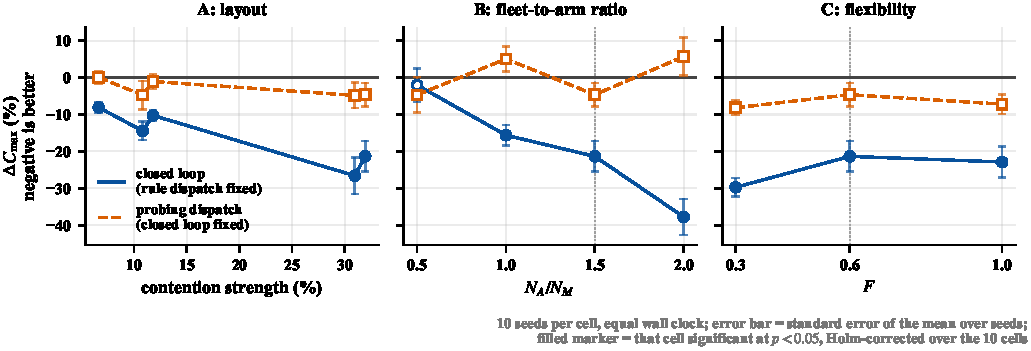
\includegraphics[width=\columnwidth]{fig/fig_prediction3.pdf}
\Description{Three panels of line plots: closed-loop gain and reservation-aware
dispatch gain across layout (vs contention), fleet-to-arm ratio, and flexibility. After
Holm correction over the ten cells the closed-loop curve is filled, hence
significant, at nine of ten cells, while the dispatch curve is hollow at every
cell, and its sign alternates across the four fleet-ratio levels. Error bars
give the standard error of the mean over the ten seeds of each cell; the
dispatch bars cross zero at every cell and the closed-loop bars do not.}
\caption{Closed-loop and dispatching gains on the three families.
Left: layout versus contention intensity; middle: $N_A/N_M$; right: flexibility.
Hollow vertical lines mark the shared base point \texttt{A funnel}.
A filled marker remains significant after Holm correction over the $\NCases$ instances of that effect; a hollow marker does not.
Error bars are the SEM of pairwise relative gains over $\NSeeds$ seeds.
Read whether each curve can be distinguished from zero, not the shape of the dispatching curve.}
\label{fig:prediction3}
%% From fig/fig_prediction3.py and baseline_ladder.csv.
%% x-axis: Family A uses contention intensity; B/C use the factor level in the
%% instance name (written by abc_matrix).  Shared base A funnel has no level in
%% the name; the script fills (1.5, 0.6) from abc_matrix.BASE.
%% Filled/open markers follow Holm p over the ten instances of that effect
%% (not the current panel).  The dispatching curve is all open.
\end{figure}

\emph{Layout.}
The closed loop is significant on all five instances and rises roughly with contention: \GainLoopScatter{} on \texttt{scatter} (\ContentionLo{}), \GainLoopMid{}/\GainLoopLow{} on \texttt{mid}/\texttt{low}, \GainLoopFunnel{}/\GainLoopHigh{} on \texttt{funnel}/\texttt{high}.
Two inversions block a monotone ranking.
\texttt{low} versus \texttt{mid} crosses the grid/dumbbell boundary of Section~\ref{sec:instances} (\LegGrid{} versus \LegDumbbell{}) and is not a pure contention contrast.
\texttt{funnel} versus \texttt{high} differs only by one station lane---the designated cleanest contrast---and is the inversion that is a counter-example.
What remains is the span (\GainLoopFunnel{} versus \GainLoopScatter{}, about two and a half times), not an ordering; contention intensity does not say how much wait can be bypassed by reassignment (limitation~(1) of Section~\ref{sec:limitations}).
Dispatching is not significant on any instance of this family; four of five signs match the closed loop.

\emph{Vehicle-to-arm ratio.}
This family does not determine an upper bound of applicability for dispatching.
Dispatching at the four levels is $-\GainProbeStarve$ ($0.5$), \GainProbeFleetOne{} ($1.0$), \GainProbeFleetBase{} ($1.5$), \GainProbeFleetTwo{} ($2.0$): the sign alternates, and none is significant even before correction ($p\PProbeFleetHalfRaw$, $p\PProbeFleetOneRaw$, $p\PProbeFleetBaseRaw$, $p\PProbeFleetTwoRaw$).
Without the base point the curve would show the monotone rise predicted by the cost law; when an effect is of the same order as per-instance noise, subset selection alone can produce a spurious trend.
The cost-law upper bound of Section~\ref{sec:costlaw} therefore remains untested.
The closed loop at $1.0$ and $2.0$ is \GainLoopFleetOne{} and \GainLoopFleetTwo{}, both significant: fleet size mainly affects the closed-loop gain, not dispatching.

\emph{Flexibility.}
After Holm correction, dispatching is not significant in this family either.
At $F=0.3$, $0.6$, and $1.0$ the gains are \GainProbeFlexLo{}, \GainProbeFleetBase{}, and \GainProbeFlexHi{}, all of the same sign; the two ends are the largest among the $\NCases$ instances but are no longer significant after correction ($p\PProbeFlexLoHolm$, $p\PProbeFlexHiHolm$), so the family provides directional evidence only.
The same sign at $F=0.3$, where the room for reassignment is smallest, is compatible with dispatching acting mainly through vehicle selection and timing rather than through reassignment to another arm.
The closed loop is \GainLoopFlexLo{} and \GainLoopFlexHi{}, still significant per instance after correction.

\paragraph{An independent batch, and heterogeneity is not an amplifier.}
A contended cross-check ($\MatrixCells$ instances $\times$ $10$ seeds, two-stage surrogate baseline, per-instance wall-clock $30.2$--$72.9$\,s) gives an integration gain of \GainIntegMatrix{}, significant on \SigIntegMatrix{} instances (uncorrected counts from that batch; the second exception of Section~\ref{sec:protocol}), from \GainIntegMatrixLo{} to \GainIntegMatrixHi{}.
By $H$ bin the same gain is \GainIntegHZero{} at $H=0$, \GainIntegHLow{} at $0.15$ (measured \MatrixHMeasLow{}, near the public median \PubHMed{}), \GainIntegHMid{} at $0.3$, and \GainIntegHHigh{} at $0.5$; the rank correlation is a weakly negative \RhoIntegH{}.
$H$ above the literature range did not inflate the closed-loop gain; $H=0$ is the highest bin, consistent with Section~\ref{sec:features}.
Dispatching on that batch is \GainProbePre{}, significant on $0$ instances; the most likely reason is that the batch ran before the speed-ups of Section~\ref{sec:speedup} (Section~\ref{sec:costlaw}).

